\documentclass[journal]{vgtc}                % final (journal style)
%\documentclass[review,journal]{vgtc}         % review (journal style)
%\documentclass[widereview]{vgtc}             % wide-spaced review
%\documentclass[preprint,journal]{vgtc}       % preprint (journal style)
%\documentclass[electronic,journal]{vgtc}     % electronic version, journal

%% Uncomment one of the lines above depending on where your paper is
%% in the conference process. ``review'' and ``widereview'' are for review
%% submission, ``preprint'' is for pre-publication, and the final version
%% doesn't use a specific qualifier. Further, ``electronic'' includes
%% hyperreferences for more convenient online viewing.

%% Please use one of the ``review'' options in combination with the
%% assigned online id (see below) ONLY if your paper uses a double blind
%% review process. Some conferences, like IEEE Vis and InfoVis, have NOT
%% in the past.

%% Please note that the use of figures other than the optional teaser is not permitted on the first page
%% of the journal version.  Figures should begin on the second page and be
%% in CMYK or Grey scale format, otherwise, colour shifting may occur
%% during the printing process.  Papers submitted with figures other than the optional teaser on the
%% first page will be refused.

%% These three lines bring in essential packages: ``mathptmx'' for Type 1
%% typefaces, ``graphicx'' for inclusion of EPS figures. and ``times''
%% for proper handling of the times font family.

\usepackage{mathptmx}
\usepackage{graphicx}
\usepackage{times}
\usepackage{epstopdf}
\usepackage{paralist}
\usepackage[tight]{subfigure}
\usepackage[usenames, dvipsnames]{color}
\usepackage{textcomp}
\usepackage{program}
\usepackage{stfloats}
\usepackage[table]{xcolor}
\usepackage{array}
\usepackage{ragged2e}
\usepackage{float}
\usepackage{tabularx}
\usepackage{pifont}
\usepackage{booktabs}

%% We encourage the use of mathptmx for consistent usage of times font
%% throughout the proceedings. However, if you encounter conflicts
%% with other math-related packages, you may want to disable it.

%% This turns references into clickable hyperlinks.
\usepackage[bookmarks,backref=true,linkcolor=black]{hyperref} %,colorlinks
\hypersetup{
  pdfauthor = {},
  pdftitle = {},
  pdfsubject = {},
  pdfkeywords = {},
  colorlinks=true,
  linkcolor= black,
  citecolor= black,
  pageanchor=true,
  urlcolor = black,
  plainpages = false,
  linktocpage
}

\definecolor{darkGreen}{RGB}{0, 100, 0}
\definecolor{nmGreen}{RGB}{225, 255, 194}
\definecolor{nmOrange}{RGB}{254, 225, 194}
\definecolor{nmYellow}{RGB}{255, 255, 208}

\newcommand*\rot{\rotatebox{90}}
\newcommand*\OK{\ding{51}}

\newcommand*\match{\textcolor{darkGreen}{\ding{52}}}
\newcommand*\mismatch{\textcolor{red}{\ding{54}}}
\newcommand*\posmatch{\textcolor{blue}{{\bf ?}}}

\newcommand{\bstart}[1]{\vspace{1mm} \noindent{\textbf{#1:}}}

\newcommand{\bqstart}[1]{\vspace{1mm} \noindent{\textbf{#1}}}

\newcommand{\bscstart}[1]{\vspace{1mm} \noindent{\sc{\textbf{#1:}}}}

\newcommand{\tm}[1]{\textcolor{red}{#1}}
\newcommand{\mb}[1]{\textcolor{blue}{#1}}

\newcommand{\etal}{et al.}
\newcommand{\eg}{e.\ g.}
\newcommand{\ie}{i.\ e.}

%% If you are submitting a paper to a conference for review with a double
%% blind reviewing process, please replace the value ``0'' below with your
%% OnlineID. Otherwise, you may safely leave it at ``0''.
\onlineid{0}

%% declare the category of your paper, only shown in review mode
\vgtccategory{Research}

%% allow for this line if you want the electronic option to work properly
\vgtcinsertpkg

%% In preprint mode you may define your own headline.
%\preprinttext{To appear in IEEE Transactions on Visualization and Computer Graphics.}

%% Paper title.

\title{From Energy Analysis in Commercial Building Portfolios to Guidelines for Multiple Time-Series Visualization}

%% This is how authors are specified in the journal style

%% indicate IEEE Member or Student Member in form indicated below
\author{Matthew Brehmer, Jocelyn Ng, Kevin Tate, and Tamara Munzner,~\textit{Member, IEEE}}
\authorfooter{
%% insert punctuation at end of each item
\item
 Matthew Brehmer and Tamara Munzner are with the University of British Columbia. E-mail: \{brehmer,tmm\}@cs.ubc.ca.
\item
 Jocelyn Ng and Kevin Tate are with EnerNOC, Inc. E-mail: \{jocelyn.ng,kevin.tate\}@enernoc.com.
}

%other entries to be set up for journal
\shortauthortitle{Biv \MakeLowercase{\textit{et al.}}: From Energy Analysis to Multiple Time-Series Visualization Guidelines}
%\shortauthortitle{Firstauthor \MakeLowercase{\textit{et al.}}: Paper Title}

%% Abstract section.
\abstract{
The energy performance of a portfolio of commercial buildings is difficult to monitor and analyze, as current analysis tools used in this domain are either not scalable or present derived and aggregated data that is too coarse.
In partnership with a commercial energy analysis software development company, we conducted a visualization design study, beginning with a thorough work domain analysis and a characterization of data and task abstractions.
We describe generalizable visualization design choices framed in terms of \textsl{matches} and \textsl{mismatches} with reference to to the \textsl{Nested Blocks and Guidelines Model}~\cite{Meyer2013}, choices that are transferable beyond the energy analysis domain. 
We also present guidelines pertaining to the themes of \textsl{familiarity} and \textsl{trust}, as well as methodological considerations for visualization design projects in corporate settings, and especially those with internal collaborators their and external clients.
As a result of our research, our designs were adopted by our collaborator into their production timeline of a commercial energy analysis application that will soon be deployed to hundreds of thousands of customers.
} % end of abstract

%% Keywords that describe your work. Will show as 'Index Terms' in journal
%% please capitalize first letter and insert punctuation after last keyword
\keywords{Design study, redesign, energy analysis, task and requirements analysis, time-series data.}

%% ACM Computing Classification System (CCS). 
%% See <http://www.acm.org/class/1998/> for details.
%% The ``\CCScat'' command takes four arguments.

\CCScatlist{ % not used in journal version
 \CCScat{H.5.2}{Information Interfaces and Presentation (e.g. HCI)}{User interfaces}{Graphical user interfaces (GUI), Evaluation/methodology, User-centered design}
}

%% Uncomment below to include a teaser figure.
%   \teaser{
%   \centering
%   \includegraphics[width=16cm]{CypressView}
%   \caption{In the Clouds: Vancouver from Cypress Mountain.}
%   }

%% Uncomment below to disable the manuscript note
%\renewcommand{\manuscriptnotetxt}{}

%% Copyright space is enabled by default as required by guidelines.
%% It is disabled by the 'review' option or via the following command:
% \nocopyrightspace

%%%%%%%%%%%%%%%%%%%%%%%%%%%%%%%%%%%%%%%%%%%%%%%%%%%%%%%%%%%%%%%%
%%%%%%%%%%%%%%%%%%%%%% START OF THE PAPER %%%%%%%%%%%%%%%%%%%%%%
%%%%%%%%%%%%%%%%%%%%%%%%%%%%%%%%%%%%%%%%%%%%%%%%%%%%%%%%%%%%%%%%%

\begin{document}

%% The ``\maketitle'' command must be the first command after the
%% ``\begin{document}'' command. It prepares and prints the title block.

\maketitle

%% the only exception to this rule is the \firstsection command
%% \section{Introduction} %for journal use above \firstsection{..} instead

%-------------------------------------------------------------------------
%-------------------------------------------------------------------------

\section{Introduction}
\label{introduction}

%-------------------------------------------------------------------------
%-------------------------------------------------------------------------

This is a visualization design study, where visualization is used to analyze the energy performance of portfolios of dozens to hundreds of commercial buildings. 
Furthermore, this is a redesign study, which took place in collaboration with a company that develops commercial energy analysis and reporting software.

Our industry collaborator's goal in this project was to deploy a redesigned energy analysis software tool, called {\it Energy Manager}, to retain existing clients, to attract new ones, and to increase engagement. 
Thousands of energy workers had access to {\it Energy Manager}, though less than 300 were engaged and actually using the tool. 
As a result of a result partnering with a large utility company, the number of potential users will increase to potentially hundreds of thousands of individuals.

Our goal as researchers in this project was to convince our collaborators to commit software development resources and adopt and the visualization designs that we put forward, those based on user research and our knowledge of the visualization design space.

So why does this design study matter for an information visualization research audience?
First, this project required the design of visualizations for bar and line chart crowd. 
In other words, we needed to promote sophisticated visual analysis by potentially unsophisticated users.
This project also involved working with a variety of stakeholders in a corporate non-research setting. 
This paper documents a success story where our industry collaborator adopted some of our designs, as well as our methodology that led to this success.

\bstart{Contributions} our primary contribution is a set of generalizable visualization design choices and guidelines framed in terms of {\bf matches} and {\bf mismatches} between techniques and abstractions, guidelines that extend beyond the energy analysis domain.
We also present guidelines that relate to {\bf familiarity}, balancing familiar visualization designs with visual encodings that prospective user may have never seen before; as well as {\bf trust}, which relates to the appropriate display of derived and aggregated data, and giving users control over these data transformations.
And finally we contribute {\bf methodological advice} for visualization design projects in an industry context where prospective users include both the industry collaborator's employees and their remote external clients.

\bstart{Outline} we begin by describing the commercial energy domain in Section~\ref{domain}.
We then characterize the data and tasks in Section~\ref{abstractions}; we consider how the three tasks we characterized are supported by the existing {\it Energy Manager} tool in Section~\ref{existing-tool}, and how previous work addresses similar data and tasks in Section~\ref{related-work}.
In Section~\ref{design}, we present our designs and characterize them in terms of {\bf matches} and {\bf mismatches} for the three tasks.
The result of our design process, the adoption of our visualization designs into production, are described in Section~\ref{production}.
In Section~\ref{discussion}, we reflect on the themes of {\bf familiarity} and {\bf trust}, as well as on methodological considerations for visualization design studies in corporate settings.
Finally, Section~\ref{conclusion} summarizes our contributions.

%-------------------------------------------------------------------------
%-------------------------------------------------------------------------

\section{Domain Background}
\label{domain}

%-------------------------------------------------------------------------
%-------------------------------------------------------------------------

As in many design study papers, it's helpful to provide a little domain background to the reader before launching into abstractions and design~\cite{Brehmer2014a,Lloyd2011,McNamara2014,Vicente1999}.

\bstart{Work domain analysis} in order to understand the energy work domain, we began by speaking to energy workers, and focused on workers who oversee portfolios of many buildings.
We conducted 9 in-depth interviews in 2013 with current users of {\it Energy Manager}, our collaborator's software, which had over 200 active users (thousands of users had access). 
Most were clients of our collaborator, and one was an employee of our collaborator. 
Some of these interviews took place locally, others were done via Skype, as most clients of our collaborator are located in other cities or countries.
We found a wide range in terms of roles, job titles, skill sets, levels of training, and the tools that were used, which included {\it Energy Manager}; to which we inquired about its context and frequency of use.

\bstart{Domain goals and activities} though the energy workers we interviewed reported a range of roles and responsibilities, there were some common goals and activities.
These individuals oversaw the energy performance of portfolios of dozens to hundreds of buildings, such as a school board, a university, or a hotel chain. 
They needed to balance a need to reduce costs and conserve energy while ensuring the comfort and safety of people who used the buildings.
To achieve these goals, the energy workers would need to (1) assess the performance of buildings in their portfolio following an energy conservation measure, such as installing new windows or lighting, (2) determine which buildings in their portfolio require energy conservation measures, and (3) find and diagnose anomalous energy performance such as spikes, outages, surges, or otherwise erratic and inconsistent energy performance.

%-------------------------------------------------------------------------
%-------------------------------------------------------------------------

\section{Abstractions}
\label{abstractions}

%-------------------------------------------------------------------------
%-------------------------------------------------------------------------

\begin{figure}[t]
    % \vspace{-0.6cm}
	\centering
	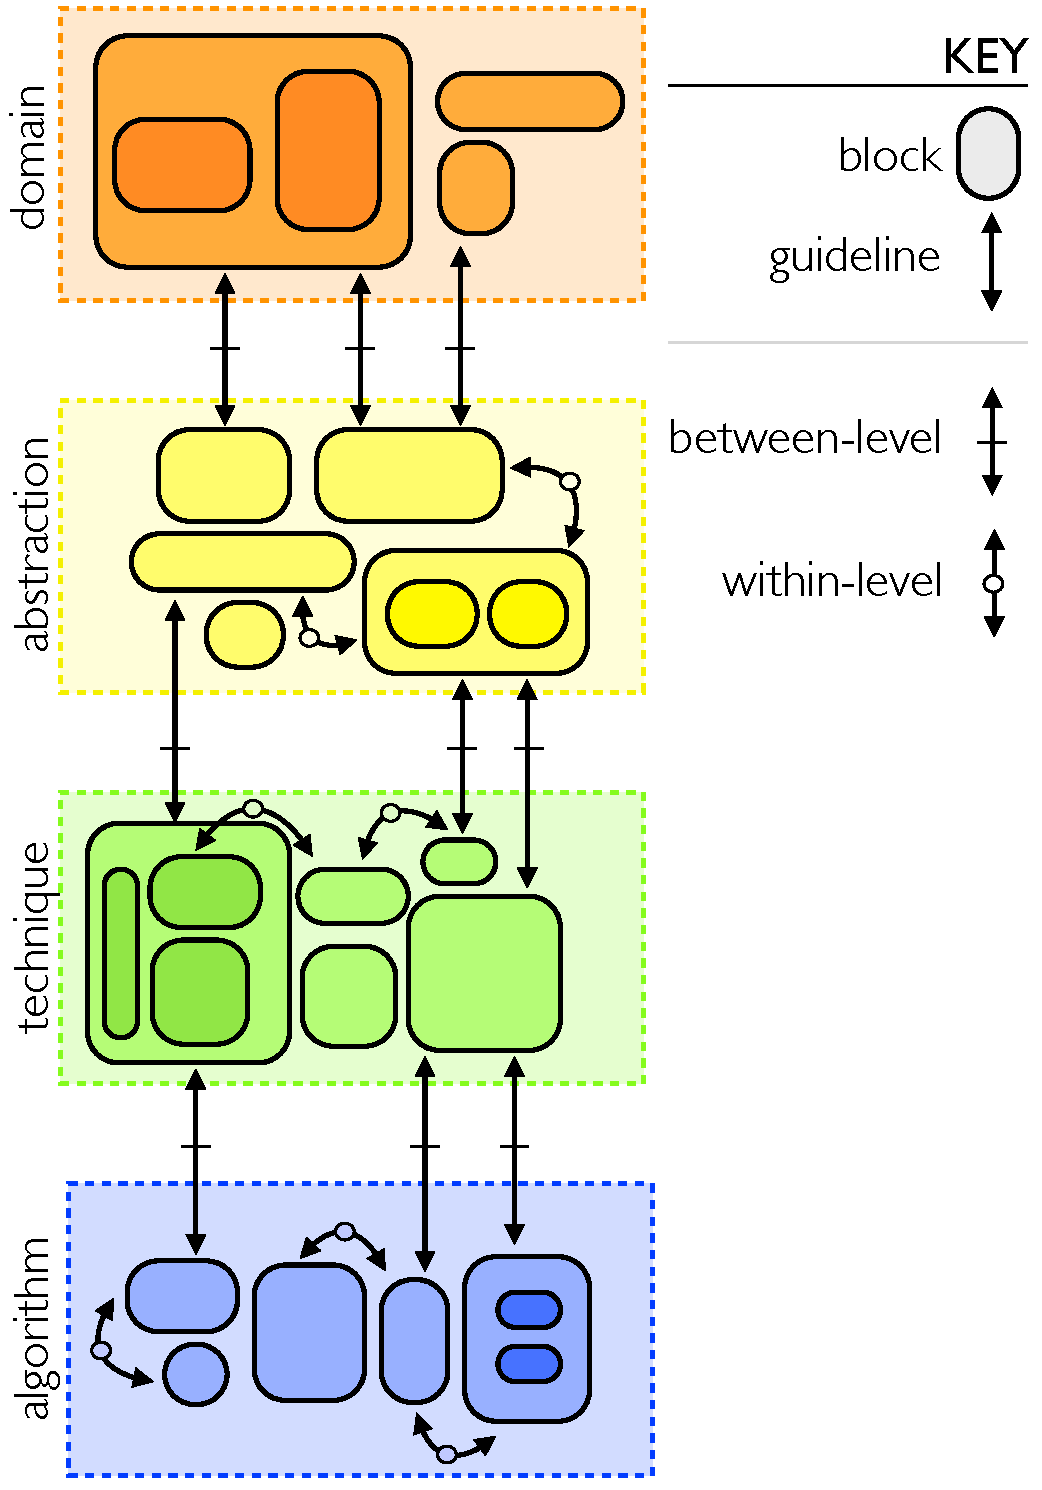
\includegraphics[width=0.67\columnwidth]{figures/blocks-and-mappings.pdf}
	\vspace{-0.3cm}
	\caption{The \textsl{nested blocks and guidelines model}~\cite{Meyer2013}. We propose \textsl{guidelines} framed in terms of \textsl{matches} and \textsl{mismatches} between abstraction \textsl{blocks} and idiom \textsl{blocks}.}
	\label{fig:nested-model}
	\vspace{-0.6cm}
\end{figure} 

Now let's characterize these domain problems in terms of data and task abstractions.

%-------------------------------------------------------------------------

\subsection{Data Abstraction}
\label{data-abstractions}

%-------------------------------------------------------------------------

We begin with characterizing the data.

\begin{table}[ht]\renewcommand{\arraystretch}{1.2}\addtolength{\tabcolsep}{-1pt}
    \vspace{-.3cm}
    \begin{center}
    \scriptsize
    \begin{tabular}{l|l|l}

        \rowcolor{red!15}
    
        {\bf Term} & {\bf Abstraction} & {\bf Example}
    
        \\
        
        \hline
        
        \multicolumn{3}{c} {\it Building metadata} 
        
        \\
    
        \hline
        
        Building ID & unique categorical & \#123
    
        \\
        
        \rowcolor{gray!15}
        
        Building area & quantitative & 450 m$^{2}$
    
        \\
        
        Building age & quantitative & 20 years
    
        \\
        
        \rowcolor{gray!15}
        
        No. occupants & quantitative & 50 people
    
        \\
        
        Location & spatial & 49.25$^{\circ}$ N, 123.10$^{\circ}$ W
    
        \\
        
        \rowcolor{gray!15}  
        
        Tag & categorical & {\it ``restaurant''}
    
        \\
        
        \hline
        
        \multicolumn{3}{c} {\it Temporal data for each building} 
        
        \\
    
        \hline
        
        Energy demand & quantitative & 200 kW
    
        \\
        
        \rowcolor{gray!15}
        
        Outside temperature & quantitative & 18$^{\circ}$ C
    
        \\
        
        Open / closed & categorical & Open Mon--Fri, 08-18h
    
        \\
        
        \hline
        
        \multicolumn{3}{c} {\it Derived temporal data for each building} 
        
        \\
    
        \hline
        
        Consumption & quantitative & 800 kWh
    
        \\
        
        \rowcolor{gray!15}
        
        Energy intensity & normalized quantitative & 1.78 kWh / m$^{2}$
    
        \\
    
        Weather-independent & normalized quantitative & 200 kWh / HDD$^\ddagger$
    
        \\ 
        
        performance$^\dagger$ & & (Heating Degree Days)
        
        \\
        
        \rowcolor{gray!15}
        
        Predicted perform.$^\dagger$ & quantitative & 190 kW
        
        \\
        
        Relative differential & normalized quantitative & -- 40\%
        
        \\
        
        Rank & ordinal & 1st, 2nd, 3rd
        
        \\
        
        \hline  
        
    \end{tabular}
    \vspace{-0.3cm}
    \caption{A summary of the data abstractions. $^\dagger$\textsl{Performance} could be \textsl{demand}, \textsl{consumption}, or \textsl{intensity}. $^\ddagger$Heating and Cooling Degree Days (HDD, CDD) are derived aggregate values relative to temperature thresholds where a building's heating or cooling system is activated.}
    \label{tab:data-abstractions}
    \end{center}
    \vspace{-0.6cm}
\end{table}

\bstart{Categorical, quantitative, and spatial metadata} each building is an item with a unique identifier. 
It had quantitative attributes such as its area, age, and number of occupants; each building has a location; each building has a potentially arbitrary number of categorical attributes or tags; consider a university, where buildings are differentiated by type, like classroom or laboratory, differentiated by campus or department, like chemistry and physics, or differentiated by the name of the building operations staff responsible for the building. 

\bstart{Item groups} Since we're interested in portfolios of many buildings, we can have groupings of buildings using these attributes. 
A portfolio may have many alternative groupings, and they may overlap.

\bstart{Multiple time-series / building} the energy performance of each of those buildings is being monitored over time and time of course is both sequential and cyclic.
So in effect we have a multidimensional table of buildings, building attributes, and quantitative attributes changing over time.
The energy performance of each building has multiple time series associated with it, such as the electricity demand, the outside air temperature, whether the building is open or closed; the latter is important because we're speaking about commercial buildings.

\bstart{Derived data} the raw electricity demand or temperature time series can be helpful for detailed investigations of single buildings. 
It is more often the case that individuals performing energy analysis activities are looking at {\bf derived} and {\bf aggregated} data. 
These include {\bf averages}, {\bf minimums}, {\bf maximums}, and {\bf sums} for different time periods of interest, such as average weekday electricity demand in January.
{\bf Consumption} is the most common derived attribute, which is an accumulated amount of energy.
{\bf Intensity} is consumption normalized by buildings area, which allows you to compare the energy performance of buildings of different size.
Similarly, it's possible to {\bf normalize} energy performance values further by considering outdoor temperature, which allows you to compare buildings at different times of the year or buildings in different climate zones.
{\bf Predicted energy performance} based on statistical models are also considered, though these are problematic for reasons we describe in Section~\ref{existing-tool}.
{\bf Relative} and {\bf absolute differences} from the observed energy performance and the predicted or historical performance are also important; for example, you could determine how much better or worse a building is performing relative to last year.
And finally, given any of these derived values, you can create a {\bf ranking} to answer questions like {\it ``which are the top 5 worst performing buildings in my portfolio?''}.

%-------------------------------------------------------------------------

\subsection{Task Abstractions}
\label{task-abstractions}

%-------------------------------------------------------------------------

Let's move on now to the task abstractions.

\begin{table*}[bp]\renewcommand{\arraystretch}{1.2}\addtolength{\tabcolsep}{-1pt}
    \vspace{-.3cm}
    \begin{center}
    \scriptsize
    \begin{tabular}{p{0.125\textwidth}|>{\RaggedRight}p{0.15\textwidth}|>{\RaggedRight}p{0.15\textwidth}|>{\RaggedRight}p{0.15\textwidth}|>{\RaggedRight}p{0.15\textwidth}|>{\RaggedRight}p{0.15\textwidth}}

        \rowcolor{nmYellow}
    
        {\bf Task} & \cellcolor{nmOrange} {\bf Domain activities} & {\bf Scope} & {\bf Abstraction: {\tt Actions}} & {\bf Abstraction: {\tt Targets}} & {\bf Example}
        
        \\
        
        \hline  
        
        %task name
        \cellcolor{nmYellow} {\bf T1}: Overview 
        
        %domain activities
        & \cellcolor{nmOrange} Determine which building(s) require energy conservation measures. Find anomalous energy performance.
        
        %scope
        & The entire portfolio of buildings, coarser time periods. 
        
        %abstraction: actions
        & {\it consume}: {\tt discover}, {\tt present}, {\tt enjoy}; {\it search}: {\tt lookup}; {\it query}: {\tt summarize}.
        
        %abstraction: targets
        & {\it all data}: {\tt trends}, {\tt outliers}; {\it attributes}: {\tt distributions}, {\tt extremes}, {\tt similarities}. 
        
        %example question
        & {\it ``How did my building portfolio perform this past year?''}
        
        \\
        
        \hline
        
        %task name
        \cellcolor{nmYellow} {\bf T2}: Detail 
        
        %domain activities
        & \cellcolor{nmOrange} Assess performance following energy conservation measures. Find and diagnose anomalous energy performance. 
        
        %scope
        & Groups of buildings within the portfolio, finer time periods.
        
        %abstraction: actions
        & {\it consume}: {\tt discover}; {\it search}: {\tt locate}; {\it query}: {\tt compare}. 
        
        %abstraction: targets
        & {\it all data}: {\tt trends}, {\tt outliers}, {\tt features}.
        
        %example question
        & {\it ``Are my restaurants in Vancouver performing better this January than they did last January?''}
        
        \\
        
        \hline
        
        %task name
        \cellcolor{nmYellow} {\bf T3}: Proportion 
        
        %domain activities
        & \cellcolor{nmOrange} Find and diagnose anomalous energy performance. 
        
        %scope
        & Groups of buildings within the portfolio, finer time periods. 
        
        %abstraction: actions
        & {\it consume}: {\tt discover}; {\it search}: {\tt locate}, {\it explore}; {\it query}: {\tt identify}. 
        
        %abstraction: targets
        & {\it all data}: {\tt trends}, {\tt outliers}, {\tt features}; {\it attributes}: {\tt dependencies}. 
        
        %example question
        & {\it ``What proportion of my university’s energy consumption is consumed by its computer science building over time?''}
        
        \\
        
        \hline  
        
    \end{tabular}
    \vspace{-0.3cm}
    \caption{A summary of the task abstractions (yellow) and their corresponding domain activities (orange). The task abstractions are characterized according to a recent task typology~\cite{Brehmer2013}, distinguishing between \textsl{actions} and \textsl{targets}~\cite{Munzner2014}.}
    \label{tab:task-abstractions}
    \end{center}
    \vspace{-0.6cm}
\end{table*}

We characterized the task abstractions in this project using a recent task typology~\cite{Brehmer2013}, distinguishing between actions and targets~\cite{Munzner2014}.

\bstart{T1 / Overview} the first task, Overview, is one in which the analyst performs a {\tt lookup} and {\tt summarizes} all the items over a period of time, and this corresponds to the domain activities of determining which buildings in the portfolio require energy conservation measures and finding anomalous energy performance. 
{\tt Trends}, {\tt outliers}, {\tt distributions}, {\tt extreme values}, and {\tt similarities} are of interest. 
An example question would be {\it ``How did my building portfolio perform this past year?''}.

\bstart{T2 / Detail} the second task is the result of drilling down from the portfolio to a group of buildings, examining performance in detail: {\tt locating} and {\tt comparing} data from groups of items over time, corresponding to the domain activities of assessing building performance following energy conservation measures, or finding and diagnosing anomalous energy performance. 
An example question would be {\it ``Are my restaurants in Vancouver performing better this January than they did last January?''}.

\bstart{T3 / Proportion} finally, the third task is the converse of drilling down, as once you've gone from portfolio to group, this task is about {\tt locating} and {\tt exploring} to {\tt identify} the proportion of individual energy use from individual items relative to the group.
An example question would be {\it ``what proportion of a university campus's energy consumption is consumed by its computer science building over time?''} or {\it ``what building on the campus consumes the largest proportion of energy?''}.

\bstart{Task sequences} as you might have guessed, these tasks are not performed in isolation but in sequence. 
However, some sequences occur more often than others. 
It's common for energy workers to skip the Overview ({\bf T1}) task; she or he may have a direct question about a subset of items and proceed directly to the Detail ({\bf T2}) or Proportion ({\bf T3}) task. 
You'll also notice the cycling between Detail ({\bf T2}) and Proportion ({\bf T1}) tasks, as answers from one tend to lead to new questions.

%-------------------------------------------------------------------------
%-------------------------------------------------------------------------

\section{Existing Tool}
\label{existing-tool}

%-------------------------------------------------------------------------
%-------------------------------------------------------------------------

Now that we have characterized the data and task abstractions, we can analyze existing tools and related work and determine the extent to which the tasks are supported.

%figure: energy manager screenshots

We focus on {\it Energy Manager} first, our collaborator's existing software, which all of the energy workers we interviewed had used to a varying extent for performing portfolio energy analysis.

{\it Energy Manager} is a multiple-page, multiple-view web-based application.
A summary dashboard is shown in the main page (the larger image on the right). 
Those that we interviewed used this sparingly, if at all. 
More detailed line and bar charts such as those shown on the left are indexed on the other pages, similar to how Microsoft {\it Excel} has workbooks, pages, and charts. 
Unlike {\it Excel}, the visualizations here have some interactivity, such as zooming, panning, and mouse-over performance. 
However, none of the visualizations are linked to one another or to the dashboard, so you have to navigate between them manually.

\bstart{Analysis} {\it Energy Manager} uses a small number of visualization idioms: bar charts and grouped bar charts are used for derived aggregate values such as consumption, while superimposed line charts are used for continuous values such as demand. 
At the bottom is a sortable table listing relative and absolute differential values, consumption, and intensity, aggregated over a period of time. 
None of the energy workers that we interviewed reported to have found this table useful.

{\it Energy Manager} only partially supports the Overview ({\bf T1}) task: you can look at the aggregate consumption for the portfolio over time, or alternatively you can read aggregate values in the sortable table, but you can't see variation over time across individual items. 
The Detail ({\bf T2}) task is supported but current solutions don't scale, especially since superimposed line charts and grouped bar charts are limited in terms of the number of available colours you can use when the number of items is large. 
The Proportion ({\bf T3}) task isn't explicitly supported, though its possible in some cases to estimate proportion from bar and line charts, this tends to be error-prone.
Finally, because the visualizations in {\it Energy Manager} aren't coordinated or linked in any way, it is very difficult to perform these tasks in sequence. 
As in {\it Excel}, you have to locate an existing visualization or specify a new visualization using a wizard dialog, so if the bar or line chart for a set of items doesn't already exist when you need it, you have to create it. By the time you've created it, you may have forgotten your question.

{\it Energy Manager} covers only a small part of the visualization design space: colour encoding, ordering in sorted tables, and limited navigation.
You can select items manually when creating a line chart or bar chart, but you can't filter by shared item attributes, such as filtering a portfolio of buildings to only show restaurants.
Similarly, you can't aggregate based on shared attributes: for instance, you can't compare the aggregate energy performance of restaurants in Vancouver to those in Calgary.
Aside from the seldom-used dashboard, there is no faceting in {\it Energy Manager}: the energy workers that we interviewed reported opening many browser windows, adjusting line or bar charts to display the same scale and ranges, and tiling these windows manually.
Finally, there is no linking between visualizations, so it is difficult to drill down or alternate from Overview ({\bf T1}) to Detail ({\bf T2}) and Proportion ({\bf T3}) Tasks.
Due to these limitations, {\it Energy Manager} provides only tiny slices of the multidimensional table, or aggregations that are far too coarse to be useful.

\bstart{Interview observations} the energy workers that we interviewed varied tremendously in terms of their use of {\it Energy Manager}: how they used it and how often, some weekly or daily, some using it quarterly or biannually.
Many of those we interviewed would routinely export data from {\it Energy Manager} and import it into {\it Excel} to perform custom analysis or create custom reports.
Furthermore, those that we interviewed didn't {\bf trust} {\it Energy Manager}'s derived predicted values based on statistical models, and that comparing to historical data would be preferred.
Finally, many of the derived aggregate values presented in {\it Energy Manager} were too coarse. In other words, there was a lack of {\bf trust} as a result of this loss of detail: these derived and aggregated values may be hiding information such as extreme values and distributions.

%-------------------------------------------------------------------------
%-------------------------------------------------------------------------

\section{Related Work}
\label{related-work}

%-------------------------------------------------------------------------
%-------------------------------------------------------------------------

So how is this set of data and task abstractions addressed in related work?

\bstart{Energy visualization} before we look broadly in the visualization literature, let's consider related work in the energy domain.
Erickson~\etal~\cite{Erickson2013} recently presented a web-based residential energy dashboard for home-owners, allowing them to compare against their neighbours with {\bf familiar} bar and line charts. 
However, this didn't address the analysis work of someone overseeing a portfolio of many buildings.
More than 15 years ago, van Wijk and van Selow~\cite{vanWijk1999} presented a calendar matrix visualization for time-series data, and one use case they considered was the energy performance of a single building.
Later we'll examine how this could be extended to multiple buildings.

There are also several recent examples of using {\bf map-based visualizations} to summarize the energy performance of many buildings in a local area~\cite{Heat2014,MEP2014}.
We found through our interviews with collaborators and their clients that maps are fine for presenting coarse aggregate summary values of energy performance but not for analysis work of multiple time series, especially when the energy worker is already {\bf familiar} with the locations of buildings in their portfolio, which may span large geographic areas. 
On the other hand, maps may be an effective way to filter a building portfolio by location, which is a feature that have considered.

Most closely related to our work is that of Goodwin~\etal~\cite{Goodwin2013}, who presented a few prototype visualizations of modelled residential energy use at the device-level scale across thousands of households. 
Their tasks overlap to a degree with ours, though their designs focus on load-shifting simulations performed by energy modellers. 
Their designs included horizon charts and made heavy use of faceting and matrix encodings. 
However, the focus and main contribution of their paper was on creative methods for visualization requirements analysis, rather than on the designs themselves.

\bstart{Multiple time-series visualization} Stepping back from the energy domain, there is quite a bit of related work in the visualization literature about visualizing multiple time series. 
Many of the techniques for doing so are summarized in the 2011 survey by Aigner~\etal~\cite{Aigner2011}.

There are also design studies in other domains that involve multiple time series that focus on scalability, such as {\it Line Graph Explorer}~\cite{Lam2007} and {\it LiveRAC}~\cite{McLachlan2008}. 
However, these pertain to continuous time series, while our work examines both continuous values such as energy demand, as well as discrete aggregated values.

%-------------------------------------------------------------------------
%-------------------------------------------------------------------------

\section{Design and Evaluation}
\label{design}

%-------------------------------------------------------------------------
%-------------------------------------------------------------------------=

We're now ready to dive into the visualization design.

%figure: annotated sandbox

\bstart{An energy portfolio visualization sandbox} in this project, we developed an interactive visualization design sandbox, one where we could easily prototype different visualization designs. 
Most of the designs in the following slides were produced within this interactive environment, which was developed using RStudio's Shiny web application framework\footnote{\url{shiny.rstudio.com}}.
Most importantly, we put interactive controls for filtering, aggregating, unit selection, and normalization front and centre in the interface, as these options were largely absent from {\it Energy Manager}.
We deployed this visualization sandbox environment on our collaborator's local intranet. 
It is also accessible publicly\footnote{\url{mattbrehmer.shinyapps.io/PortfolioSandbox} \\username: {\tt ieeevis}; password: {\tt vis2015}}, though we had to use a small anonymized dataset for the latter due to client privacy concerns.

\bstart{Nested blocks and guidelines} we'll discuss the visualizations themselves with respect to the Nested Blocks and Guidelines Model by Meyer~\etal~\cite{Meyer2013}. 
We've already described the relationship between domain activity blocks, and the data and task abstraction blocks. 
Now we'll consider the space of techniques and highlight guidelines for matching technique blocks to abstraction blocks. 
Since the space of possible techniques that we know of is large, we considered a few of them, implemented a subset of these, and ultimately selected a few good matches based on evaluation that coincided with design~\cite{Sedlmair2012}.

\bstart{Matches \& mismatches} we identified five matches between tasks ({\bf T1--T3}) and visualization techniques. 
We also identified four mismatches and one potential match. 
In the following subsections we explain the techniques we chose as well as why they were matches or mismatches.

\bstart{Evaluation} the evidence for these matches and mismatches emanates from an evaluation that occurred alongside our design. 
During the four month development period we had weekly feedback sessions with our collaborators, two evaluation sessions with two external ``power users'' from our original set of nine interviewees. 
Two additional evaluation sessions with new prospective clients were performed in the last two months.
For each evaluation with external clients, we created a custom slide deck containing annotated screenshots from the sandbox environment, which were sent to the interviewees in advance. 
The slide decks also contained annotated mockups. 
During our Skype interviews, we would demo the visualization sandbox via screen sharing; and both slide decks and demos would their own data. 
These calls took between 60 and 90 minutes. 
We took extensive notes and in some cases recordings; we asked them both about the perceived utility of these visualizations and how they might be used in a sequential workflow. 
We later annotated these slide decks based on their comments and suggestions.
Later, we consolidated all of our findings into a master slide deck, which was presented to our collaborator as an evidence-based research summary. 
The following slides present a subset of these findings.

%-------------------------------------------------------------------------

\subsection{Faceted Visualizations for Overview and Detail Tasks}
\label{design-faceting}

%-------------------------------------------------------------------------'

%figure: faceting

We first tried to address the Overview ({\bf T1}) and Detail ({\bf T2}) tasks. 
Recall that an example Overview question is {\it ``How did my entire building portfolio perform this past year?''}, while an example Detail question is {\it ``Are my restaurants in Vancouver performing better this January than they did last January?''}.
At first we thought that faceting would be the solution for both the Overview ({\bf T1}) and Detail ({\bf T2}) tasks, to overcome the scalability issues associated with grouped bar charts and superimposed line charts.
We considered faceted bar charts, boxplots, and line graphs.

\bstart{Faceted bar charts} with bar charts, you could facet by each building or by a temporal granularity. 
However, if you have a group of dozens or hundreds of buildings, faceting will not scale. 
We determined that it was a poor match for the Overview ({\bf T1}) task, though a potential match for the Detail ({\bf T2}) task, provided that the energy worked has filtered the set of buildings to consider, like filtering from a university campus to just the ``classroom'' buildings.
In addition, one of the two power users that we interviewed stated that the bars only show one coarse aggregate values, typically an average or sum, that there was a loss of detail. 
They don't show ranges or extreme values.

\bstart{Faceted boxplots} this is why we considered faceted boxplots, to be able to compare ranges and distributions for multiple items at different points in time, such as from over the course of several months.
However, we found that most people we spoke to, both employees and clients, weren't {\bf familiar} with boxplots, except for a minority who had taken a post-secondary stats class. 
Furthermore, unlike faceted bar charts where you only need to make comparisons of position aligned to a each facet's baseline: comparisons in faceted boxplots are more difficult because you are comparing multiple positions and widths across separate facets. 
It is therefore a daunting introduction to box plots for those unfamiliar with them and a poor match for the Detail ({\bf T2}) task.

\bqstart{Faceted line charts}, however, are a good match for the Detail ({\bf T2}) task, especially with continuous quantitative time-series values such as energy demand; and they are a scalable alternative to superimposed line charts. 
Furthermore, the line chart encoding is already quite {\bf familiar} to the energy workers that we interviewed.

%-------------------------------------------------------------------------

\subsection{Overview Visualizations of Rank and Rank Change}
\label{design-ranking}

%-------------------------------------------------------------------------

%figure: bar + bump

Let's return now to that Overview ({\bf T1}) task and try something other than faceting.
Remember how the ranking table in {\it Energy Manager} was never used for the Overview ({\bf T1}) task? In that it only provided coarse aggregated values for each item for one time period.
We considered encodings for displaying rank as well as rank change over time.

\bstart{Bump plots} the first of these, a bump plot, uses a {\bf familiar} line encoding and shows rank change over time. 
The problem with this encoding is that it is difficult to distinguish items using colour, since there are only a handful of viable colours. 
Alternatively, we could highlight items by rank change or rank variation.
In addition, bump plots only show relative rank and rank change, whereas the absolute values that produce the ranks are hidden. 
As a result this a loss of detail, the bump plot is also a poor match for the Overview ({\bf T1}) task.

\bstart{Bump + bar plots} we then considered an encoding that incorporates both relative rank, rank change, and absolute value, by adding {\bf familiar} bars to each point in the bump plot series of ranks. 
This is similar to some recent related work that proposed techniques that display both relative rank and absolute value~\cite{Gratzl2013,Hur2013}. 
We still face the scalability problem associated with colour discriminability. 
A combination of interaction and highlighting by rank change or rank variation might improve this visualization.
The energy workers that we interviewed did respond well to this visualization, as it is composed of {\bf familiar} encodings: bars and lines. 
However, we came to realize that ranks as derived values are infrequently considered, perhaps only on a quarterly or annual basis, and that the bars can only convey coarse aggregates such as sums or averages. 
Therefore, the hunt for a good Overview ({\bf T1}) visualization continued.

%-------------------------------------------------------------------------

\subsection{Matrix-Based Overview Visualizations}
\label{design-matrix}

%-------------------------------------------------------------------------

%figure: matrix-based visualizations

With faceting and rank-based visualizations proving ineffective, we next turned to a matrix-based representation for the Overview ({\bf T1}) task.

\bstart{Time-series matrix} matrix representations such as these are both scalable and space-efficient.
Similar representations have been used in related work~\cite{Goodwin2013}.
These representations allow us to display observed as well as differential data, as you can see with the diverging colour scale in the bottom right matrix.
Most of the energy workers that we interviewed were {\bf unfamiliar} with this form of encoding, except one energy analyst who routinely made such visualizations in {\it Excel}. 
As a result, it took more effort to convince our collaborators of the value of matrix representations such as these.
We also initially referred to this visualization as a ``heatmap'', and this led to some confusion, as heat is already an energy-related word and the buildings have location, though this encoding does not take spatial location into account.
We also discovered that while red is fine for use in diverging colour scales, as it has a negative connotation, and is therefore inappropriate for unidirectional colour scales. 
We also learned in later interviews that users found diverging colour scales easier to read.
Because of this uncertainty, we realized that more work needed to be done.

\bstart{Calendar matrix} We extended this matrix visualization by partitioning the cells corresponding to months into calendars, and this was inspired by previous work~\cite{vanWijk1999}. 
The calendar layout is {\bf familiar} and allows us to show data at finer granularities than months, so this was very well-received by those we interviewed and served to reduce the unfamiliarity of the matrix layout.
While promising, we continued to explore this design direction.

\bstart{Matrix with auxiliary boxplots} one problem with the matrix encodings is that they convey only coarse aggregate values: averages or sums. 
Calendar partitioning is one way to show a finer resolution in the same amount of space. 
Here we complement the aggregate values in the matrix by juxtaposing boxplots encoding ranges and distributions for each row of the time series. 
Though the issue of boxplot {\bf familiarity} is unresolved, these boxplots are easier to read than faceted boxplots, and they're reinforced by data shown the matrix, which is preferable to showing boxplots in isolation. 
Together the matrix with juxtaposed boxplots is a match for the Overview ({\bf T1}) task.

%-------------------------------------------------------------------------

\subsection{Proportion Visualizations}
\label{design-proportion}

%-------------------------------------------------------------------------

%figure: proportion visualizations

Finally, now with the Overview ({\bf T1}) and Detail ({\bf T2}) tasks addressed, the Proportion ({\bf T3}) task remains. 
Recall that a typical question here could be ``what proportion of a university's energy consumption is consumed by its computer science building over time?''.

\bstart{Stacked area \& bar charts} the visualization for this task tended to be more obvious, with stacked area and stacked bar charts appearing to be ideal candidates.
However, recall that the Detail ({\bf T2}) and Proportion ({\bf T3}) tasks are often performed in alternation, so we were concerned about the loss of context when switching between stacked bar or area charts and faceted bar or line charts.

\bstart{Juxtaposed stacked and faceted visualizations} one solution could involve juxtaposing the stacked chart and the faceted charts, and provide linked highlighting between elements in the stack and those in the facets. 
As a result of this juxtaposition and linking, both the Detail ({\bf T2}) and Proportion ({\bf T3}) tasks are addressed.

%-------------------------------------------------------------------------

\subsection{Summary of Matches and Mismatches} 
\label{design-summary}

%-------------------------------------------------------------------------

\begin{table}[ht]\renewcommand{\arraystretch}{1.2}\addtolength{\tabcolsep}{-1pt}
    \vspace{-.3cm}
    \begin{center}
    \scriptsize
    \begin{tabular}{l|l|c}

        \rowcolor{gray!15}
    
        {\bf Task} & {\bf Visualization Idiom} & {\bf Match?}
        
        \\
        
        %task
        \cellcolor{nmYellow} {\bf T1}: Overview 
        
        %idiom
        & \cellcolor{nmGreen} Faceted bar chart 
        
        %match?
        & \mismatch
        
        \\
        
        %task
        \cellcolor{nmYellow} %{\bf T1}: Overview 
        
        %idiom
        & \cellcolor{nmGreen} Bump plot 
        
        %match?
        & \mismatch
        
        \\
        
        %task
        \cellcolor{nmYellow} %{\bf T1}: Overview 
        
        %idiom
        & \cellcolor{nmGreen} Bar + bump plot 
        
        %match?
        & \posmatch
        
        \\
        
        %task
        \cellcolor{nmYellow} %{\bf T1}: Overview 
        
        %idiom
        & \cellcolor{nmGreen} Map 
        
        %match?
        & \mismatch
        
        \\
        
        %task
        \cellcolor{nmYellow} %{\bf T1}: Overview 
        
        %idiom
        & \cellcolor{nmGreen} (Calendar) matrix 
        
        %match?
        & \posmatch
        
        \\
        
        %task
        \cellcolor{nmYellow} %{\bf T1}: Overview 
        
        %idiom
        & \cellcolor{nmGreen} Matrix + auxiliary boxplots 
        
        %match?
        & \match
        
        \\
        
        \hline
        
        %task
        \cellcolor{nmYellow} {\bf T2}: Detail 
        
        %idiom
        & \cellcolor{nmGreen} Faceted bar chart 
        
        %match?
        & \match
        
        \\
        
        %task
        \cellcolor{nmYellow} %{\bf T2}: Detail 
        
        %idiom
        & \cellcolor{nmGreen} Faceted boxplot 
        
        %match?
        & \mismatch
        
        \\
        
        %task
        \cellcolor{nmYellow} %{\bf T2}: Detail 
        
        %idiom
        & \cellcolor{nmGreen} Faceted line graph 
        
        %match?
        & \match
        
        \\
        
        \hline
        
        %task
        \cellcolor{nmYellow} {\bf T3}: Proportion 
        
        %idiom
        & \cellcolor{nmGreen} Stacked area graph 
        
        %match?
        & \match
        
        \\
        
        %task
        \cellcolor{nmYellow} %{\bf T3}: Proportion 
        
        %idiom
        & \cellcolor{nmGreen} Stacked bar chart 
        
        %match?
        & \match
        
        \\
        
        \hline  
        
    \end{tabular}
    \vspace{-0.3cm}
    \caption{A summary of the \textsl{matches} and \textsl{mismatches} between task abstractions and visualization idioms.}
    \label{tab:matches-mismatches}
    \end{center}
    \vspace{-0.6cm}
\end{table}

To recap, we identified five matches between tasks ({\bf T1--T3}) and visualizations. 
We also identified four mismatches and one potential match: that of a bump + bar plot for showing rank change over time; our hesitation to call this a match stems not from a problem with the visualization itself, but from energy workers' low priority on ranks as derived data.

Considering these tasks ({\bf T1--T3}), these five matches serve as generalizable guidelines that are transferable beyond the energy domain.

%-------------------------------------------------------------------------

\subsection{Interaction Design Considerations}
\label{design-interaction}

%-------------------------------------------------------------------------

You'll notice that these technique blocks are mostly about visual encodings. 
We also want to stress the importance of interaction idioms as well, namely selection, linking and brushing, filtering, aggregation, and deriving normalized values.

\bstart{Interactive auxiliary boxplots} we focused on interaction design prototyping following the visual encoding design phase, in which we focused on linking and coordinating the visualizations, such as in these prototype examples of linking and brushing to better coordinate the matrix and the boxplots. 
At the top we see subsets of the data being superimposed onto the boxplot when brushing a time period, and in the bottom we see boxplots of a subset of the time-series data shown alongside the boxplot for the entire time series. 

This interaction and linked highlighting is intended to promote engagement and facilitate the learning of both of these visual encodings, which are novel within the energy domain. These prototypes further convinced our collaborators that juxtaposing a matrix representation with linked auxiliary boxplots was a good idea.

\bstart{Linked visualizations and interactive drill-down} using visualizations created within our sandbox and drawing from feedback from the energy workers that we interviewed, we created mockups and storyboards of filtering and selection performance, to describe how an energy worker would proceed from the Overview ({\bf T1}) task to the Detail ({\bf T2}) and Proportion ({\bf T3}) tasks, otherwise known as interactive drill-down performance.

%-------------------------------------------------------------------------
%-------------------------------------------------------------------------

\section{Production (Results)}
\label{production}

%-------------------------------------------------------------------------
%-------------------------------------------------------------------------

So what was the result of all this design work? 
We had documented these matches and mismatches and presented them to our collaborator, along with our sandbox prototyping environment and mockups.
Our collaborator then ultimately decided what to implement from our prototype designs. 

%figure: energy manager ++

\bstart{Energy Manager ++} we're pleased to report that our collaborators adopted a number of our visualization designs into a new version of {\it Energy Manager}, which will soon be deployed to its large client base of potentially hundreds of thousands of users.
They made filtering and aggregation through the use of categorical building tags front and featured these prominently in the interface. 
They incorporated the matrix with auxiliary boxplots, and called it a ``site overview'', which avoids the ``heatmap'' misnomer, and matches our characterization of the Overview ({\bf T1}) task. 
They also adopted both stacked bar and area charts as well as faceted bar and line charts for the Detail ({\bf T2}) and Proportion ({\bf T3}) tasks.
They also provided linking between the visualizations, which you'll see in a moment.
Finally, they provided the ability to compare observed values against {\bf trusted} historical values, instead of or in addition to comparing observed values to less {\bf trusted} predicted values generated by a statistical model.

\bstart{Coordinated matrix \& boxplots} you'll notice the coordination between the matrix cells and boxplots, with the boxplots updating on mouseover of matrix cells. 
Our collaborators also added the ability to adjust the colour scale bounds.
Possible future work here could involve partitioning these matrix cells into calendars. 
Our collaborators intend for this visualization to be accessible on a tablet, and calendar partitioning may render these cells too small to be selectable without a fisheye zoom, which may involve a high implementation cost.

\bstart{Interactive drill-down} the other critical improvement over the original {\it Energy Manager} is the ability to drill down from a row, column, or cell of the matrix to stacked, faceted, superimposed, or individual line charts and bar charts, thereby providing a seamless drill down sequence from the Overview ({\bf T1}) task to the Detail ({\bf T2}) and Proportion ({\bf T3}) tasks.
Stacked views and faceted views are currently shown separately, though possible future work here could include juxtaposing stacks and facets, as in our prototype designs, to promote an uninterrupted alternation between the Detail ({\bf T2}) and Proportion ({\bf T3}) tasks.

%-------------------------------------------------------------------------
%-------------------------------------------------------------------------

\section{Discussion}
\label{discussion}

%-------------------------------------------------------------------------
%-------------------------------------------------------------------------

Let's step back now to go over some of the higher-level discussion points from this work.

%-------------------------------------------------------------------------

\subsection{Guidelines}
\label{discussion-guidelines}

%-------------------------------------------------------------------------

In addition to the specific guidelines regarding matches and mismatches described earlier, we propose more general guidelines relating to the themes of {\bf familiarity} and {\bf trust}.

\bstart{Familiarity} first, we learned that the juxtaposition of two unfamiliar encodings (a matrix and a boxplot) along with coordinated interaction and highlighting may facilitate learning of these novel encodings. 
Adding complexity seemed to improve interpretability. 
The same can be said about how diverging colour scales were easier to interpret that unidirectional colour scales, or how providing the ability to adjust the colour scale bounds improved matrix interpretation.
And that familiar encodings, such as bars and lines, combined in unfamiliar ways, such as in the bump and bar plot, are very quickly understood.
And finally, that visualization names themselves can be misleading: ``heatmap'' and ``boxplot'' were particular sources of confusion with those we spoke to.

\bstart{Trust} with regards to trust, we know that visualizations of derived aggregate values result in loss of detail (such as bar charts in the original {\it Energy Manager} and the cells of time-series matrix): by complementing these with visualizations of range and distribution (such as boxplots), the energy analyst gets a more complete overview of the data.
We also emphasized the need for explicit and obvious controls for filtering, aggregation, and normalization in the interface, controls that were missing in the original {\it Energy Manager}, as well as the need for alternatives to predicted values derived from statistical models that the energy workers didn't trust. 
By giving these controls to the energy worker and providing them with more agency over the creation of derived values, the derived and aggregated values are more trusted. 

%-------------------------------------------------------------------------

\subsection{Methodological Considerations}
\label{discussion-methodology}

%-------------------------------------------------------------------------

\begin{table}[ht]\renewcommand{\arraystretch}{1.2}\addtolength{\tabcolsep}{-1pt}
    \vspace{-.3cm}
    \begin{center}
    \scriptsize
    \begin{tabular}{l|*{4}l}
    
        \rowcolor{gray!15}
    
        & \multicolumn{4}{c}{\bf Artefacts}
        
        \\

        \rowcolor{gray!15}
    
        {\bf Phase} & \rot{slides, demos} & \rot{interviews} & \rot{annotations} & \rot{summary}
        
        \\
        
        \hline  
        
        (i) Work domain analysis & & \OK & & \OK
        
        \\
        
        (ii) Define and verify abstractions & \OK & \OK & \OK & \OK
        
        \\
        
        (iii) Develop visualization sandbox & \OK & & & \OK
        
        \\
        
        (iv) Evaluate visualizations, consider workflows & \OK & \OK & \OK & \OK
        
        \\
        
        (v) Prototyping specific interactions & \OK & & & 
        
        \\
        
        (vi) Production coding by collaborator & \OK & \OK & \OK &
        
        \\
        
    \end{tabular}
    \vspace{-0.3cm}
    \caption{A summary of our methodology, its phases and research artefacts.}
    \label{tab:methodology}
    \end{center}
    \vspace{-0.6cm}
\end{table}

Another point of discussion is our methodology for conducting this visualization design study in an industry setting where the stakeholders included both our collaborator and their external clients. 
These phases were referenced earlier in this talk, and this slide summarizes the phases and the research artefacts generated at each phase. Note that some of the phases overlap.

In the work domain analysis phase, we interviewed nine energy analysts and consolidated our findings in the form of notes and screenshots in an annotated slide deck.
We then validated our data and task abstractions with our collaborators and with three individuals from the original nine, this time presenting and explaining the abstractions along with screenshots and mockups containing the energy analyst's own data. 
These findings were also consolidated in a summary slide deck.

We later demoed the visualization sandbox to four clients, which included two clients who we hadn't previously spoken to, as well as internally to our collaborators, each time using the clients' own data. 
Slide decks were again used to document the designs and to record feedback as annotations on the slides. Another summary slide deck resulted from this phase.

\bstart{Stakeholder complexity} our methodology has a number of similarities and differences from Sedlmair~\etal's methodological discussion for visualization design and evaluation in corporate settings~\cite{Sedlmair2011}. 
We faced many of the same challenges identified by them. 
\mb{VERIFY: One key difference was that their discussion relates to settings where prospective users are employees of the collaborator, while in our case the target prospective users were clients of our collaborator.}

\bstart{Grounding designs in extensive qualitative analysis} we succeeded in convincing our collaborators to adopt our visualization designs as a result of the methodology we undertook. 
The rigorous user research: collecting, analyzing, and documenting of qualitative data before and during design allowed us to justify our design decisions, much in the same way that the results of a controlled experiment can justify design decisions. 
One collaborator remarked that we confirmed their earlier suspicions of what was wrong with {\it Energy Manager}, that {\it ``we performed an analysis of [{\it Energy Manager}'s] flaws in a systematic way, put a name on them, and then tested with users''}.

\bstart{Web-based visualization sandbox prototyping} there are aspects of our design and evaluation methodology that we think may generalize to other visualization design studies, especially those involving both local collaborators and their remote clients. 
For one, we used a web-based interactive sandbox prototyping environment to study matches between visualizations and tasks and to consider how the visualizations would work together in sequential workflows.

\bstart{Slide decks as research tool/artefact} we also documented all of our designs and research findings in annotated slide decks. 
Slide decks are an inherently effective way to show and explain visual encodings as well as potential interactions across slide transitions. 
They are also easy to share, especially with collaborators and external prospective users.

%-------------------------------------------------------------------------

\subsection{Future Work}
\label{discussion-future-work}

%-------------------------------------------------------------------------

This paper covered the visualization design and evaluation process until the designs left our hands and were adopted into our collaborator's production timeline.
In future work, we would like to assess the adoption of the redesigned {\it Energy Manager}, tracking usage over an extended period of time and following-up later with additional interviews and focus groups.

%-------------------------------------------------------------------------
%-------------------------------------------------------------------------

\section{Conclusion}
\label{conclusion}

%-------------------------------------------------------------------------
%-------------------------------------------------------------------------

So, to conclude this paper, we'll review the contributions.
We described generalizable visualization design choices framed in terms of {\bf matches} and {\bf mismatches} that are transferable beyond the energy analysis domain, for three tasks ({\bf T1--T3}) and a multidimensional table involving multiple time series, as well as more general guidelines pertaining to {\bf familiarity} and {\bf trust}.
We also contributed {\bf methodological guidance} for visualization design projects in a corporate setting with internal collaborators their and external clients.

As a result of our research, our designs were adopted by our collaborator into their production timeline of a commercial energy analysis application that will be deployed to hundreds of thousands of customers.

%%%%%%%%%%%%%%%%%%%%%%%%%%%%%%%%%%%%%%%%%%%%%%%%%%%%%%%%%%%%%%%%
%%%%%%%%%%%%%%%%%%%%%% END OF THE PAPER %%%%%%%%%%%%%%%%%%%%%%
%%%%%%%%%%%%%%%%%%%%%%%%%%%%%%%%%%%%%%%%%%%%%%%%%%%%%%%%%%%%%%%%%

%% if specified like this the section will be committed in review mode
\acknowledgments{
We received financial support from {\sc nserc} and Mitacs. 
We thank Cailie Crane and the {\it Energy Manager} development team, as well as the internal (collaborator) and external (client) {\it Energy Manager} users that we interviewed. 
Finally, we thank Michelle Borkin, Anamaria Cri\c{s}an, Johanna Fulda, Sung-Hee Kim, Narges Mahyar, and Joanna McGrenere for their feedback on the project and paper.
}

\bibliographystyle{abbrv}
%%use following if all content of bibtex file should be shown
%\nocite{*}
\bibliography{emu-infovis15}
\end{document}
